\section{针对连续动作的深度Q网络}

与基于策略梯度的方法相比,深度Q网络 比较稳定,策略梯度比较不稳定,玩大部分游戏不能使用策略梯度。
% 策略梯度是没有太多游戏是玩得起来的,策略梯度比较不稳,
在没有近端策略优化之前,我们很难用策略梯度做什么事情。最早 DeepMind 的论文拿深度强化学习来玩雅达利的游戏,用的就是 深度Q网络。深度Q网络 比较容易训练的一个原因是:在 深度Q网络 里面,我们只要能够估计出Q函数,就保证一定可以找到一个比较好的策略。也就是我们只要能够估计出Q函数,就保证可以改进策略。而估计Q函数是比较容易的,因为它就是一个回归问题。在回归问题里面,我们可以通过观察回归的损失有没有下降,就可以知道模型学习得好不好,所以估计Q函数相较于学习一个策略是比较容易的。我们只要估计Q函数,就可以保证现在一定会得到比较好的策略,所以一般而言 深度Q网络 比较容易操作。

但 深度Q网络 其实存在一些问题,最大的问题是它很难处理连续动作。很多时候动作是连续的,比如我们玩雅达利的游戏时,智能体只需要决定如上、下、左、右这4个动作,这种动作是离散的。很多时候动作是连续的,例如,假设智能体要开车,它要决定方向盘要左转几度、右转几度,这种动作就是连续的。
假设智能体是一个机器人,身上有 50 个 关节,它的每一个动作就对应身上 50 个关节的角度,而这些角度也是连续的。所以很多时候动作并不是离散的,它是一个向量,这个向量的每一个维度都有一个对应的值,这些值都是实数,它是连续的。如果动作是连续的,我们使用 深度Q网络 就会有困难。因为在使用 深度Q网络 时很重要的一步是我们要能够解决优化问题,也就是估计出 Q函数$Q(s,a)$ 以后,我们必须要找到一个 $a$,它可以让 $Q(s,a)$ 最大,即
\begin{equation}
  \label{eq:max_q_ch8}
  a=\underset{a}{\arg \max} Q(s, a)
\end{equation}

假设$a$是离散的,即$a$的可能性是有限的。例如,在雅达利的小游戏里面,$a$ 就是上、下、左、右与开火,它是有限的,我们可以把每一个可能的动作都代入 Q 里面算它的 Q 值。但假如$a$是连续的,我们无法穷举所有可能的连续动作,试试看哪一个连续动作可以让 Q 值最大。

怎么解决这个问题呢?我们有多种不同的方案,下面一一介绍。
\subsection{方案 1:对动作进行采样}
第1个方案是什么呢?我们可以采样出 $N$ 个可能的 $a$:$\left\{a_{1}, a_{2}, \cdots, a_{N}\right\}$ ,把它们一个一个地代入 Q函数,看谁的Q值最大。这个方案不会太低效,因为我们在运算的时候会使用 GPU,一次把 $N$ 个连续动作都代入 Q函数,一次得到 $N$ 个 Q 值,看谁最大。当然这不是一个非常精确的方案,因为我们没有办法进行太多的采样, 所以估计出来的 Q 值、最后决定的动作可能不是非常精确。
\subsection{方案 2:梯度上升}
第2个方案是什么呢?既然要解决的是一个优化问题(optimization problem),我们就要最大化目标函数(objective function)。要最大化目标函数, 我们就可以用梯度上升。我们把$a$当作参数,要找一组$a$去最大化Q函数,就用梯度上升去更新 $a$ 的值,最后看看能不能找到一个$a$最大化Q函数(目标函数)。但我们会遇到全局最大值(global maximum)的问题,不一定能够找到最优的结果,而且运算量显然很大, 因为要迭代地更新 $a$,训练一个网络就很花时间了。如果我们使用梯度上升的方案来处理连续的问题,每次决定采取哪一个动作的时候,还要训练一次网络,显然运算量是很大的。

\subsection{方案 3:设计网络架构} 
第3个方案是特别设计网络的架构,特别设计Q函数来使得解决 arg max 操作的问题变得非常容易。

如\figref{fig:fig8.2} 所示,通常输入状态 $\boldsymbol{s}$ 是图像,我们可以用向量或矩阵来表示它。
  输入 $\boldsymbol{s}$,Q函数会输出向量$\pmb{\mu}(\boldsymbol{s})$、矩阵$\pmb{\varSigma}(\boldsymbol{s})$ 和标量 $V(\boldsymbol{s})$。
  Q函数根据输入$\boldsymbol{s}$与 $\boldsymbol{a}$ 来决定输出值。到目前为止,Q函数只有输入 $\boldsymbol{s}$,它还没有输入$\boldsymbol{a}$,$\boldsymbol{a}$ 在哪里呢?接下来我们可以输入 $\boldsymbol{a}$,用$\boldsymbol{a}$与 $\pmb{\mu}(\boldsymbol{s})$、$\pmb{\varSigma}(\boldsymbol{s})$和$V(\boldsymbol{s})$ 互相作用。Q函数$Q(\boldsymbol{s},\boldsymbol{a})$可定义为
  \begin{equation}
    \label{eq:}
    Q(\boldsymbol{s},\boldsymbol{a})=-(\boldsymbol{a}-\pmb{\mu}(\boldsymbol{s}))^{\mathrm{T}} \pmb{\varSigma}(\boldsymbol{s})(\boldsymbol{a}-\pmb{\mu}(\boldsymbol{s}))+V(\boldsymbol{s})
  \end{equation}
  注意,$\boldsymbol{a}$现在是连续的动作,所以它是一个向量。假设我们要操作机器人,向量$\boldsymbol{a}$的每一个维度可能就对应机器人的每一个关节,它的数值就是关节的角度。假设 $\boldsymbol{a}$ 和 $\pmb{\mu}(\boldsymbol{s})$
  是列向量,那么 $(\boldsymbol{a}-\pmb{\mu}(\boldsymbol{s}))^{\mathrm{T}}$ 是一个行向量。$\pmb{\varSigma}(\boldsymbol{s})$ 是一个正定矩阵(positive-definite matrix),因为 $\pmb{\varSigma}(\boldsymbol{s}) = \boldsymbol{L}\boldsymbol{L}^{\mathrm{T}}$,其中 $\boldsymbol{L}$ 为下三角矩阵(lower-triangular matrix)。 $\boldsymbol{a}$-$\pmb{\mu}(\boldsymbol{s})$也是一个列向量。所以Q值即
   $-(\boldsymbol{a}-\pmb{\mu}(\boldsymbol{s}))^{\mathrm{T}} \pmb{\varSigma}(\boldsymbol{s})(\boldsymbol{a}-\pmb{\mu}(\boldsymbol{s}))+V(\boldsymbol{s})$ 是标量。
  
  我们要怎么找到一个$\boldsymbol{a}$来最大化 Q 值呢?因为 $(\boldsymbol{a}-\pmb{\mu}(\boldsymbol{s}))^{\mathrm{T}} \pmb{\varSigma}(\boldsymbol{s})(\boldsymbol{a}-\pmb{\mu}(\boldsymbol{s}))$ 一定是正的,它前面有一个负号,假设我们不看负号,所以第一项 $(\boldsymbol{a}-\pmb{\mu}(\boldsymbol{s}))^{\mathrm{T}} \pmb{\varSigma}(\boldsymbol{\boldsymbol{s}})(\boldsymbol{a}-\pmb{\mu}(\boldsymbol{s}))$ 的值越小,最终的 Q 值就越大。因为我们是把 $V(\boldsymbol{s})$ 减掉第一项,所以第一项的值越小,最后的 Q 值就越大。怎么让第一项的值最小呢?我们直接令 $\pmb{\mu}(\boldsymbol{s})$ 等于$\boldsymbol{a}$,让第一项变成 0,就可以让第一项的值最小。 因此,令 $\pmb{\mu}(\boldsymbol{s})$ 等于$\boldsymbol{a}$,我们就可以得到最大值,解决 arg max 操作的问题就变得非常容易。所以 深度Q网络 也可以用在连续的情况中,只是有一些局限:函数不能随便设置。
    
  \begin{tcolorbox}[colframe=blue!25,colback=blue!10]
    如果 $n$阶对称矩阵$\boldsymbol{A}$ 对于任意非零的$n$维向量$\boldsymbol{x}$都有 $\boldsymbol{x}^\mathrm{T}\boldsymbol{A}\boldsymbol{x}>0$,则称矩阵$\boldsymbol{A}$为正定矩阵。
    \end{tcolorbox}
  % 因为这个东西就像是高斯分布(Gaussian distribution),所以 $\mu$ 就是高斯分布的均值,$\Sigma$ 就是高斯分布的方差。
  % 但方差是一个正定(positive definite)的矩阵,怎么样让 $\Sigma$ 一定是正定的矩阵呢?
  
  % \begin{tcolorbox}[colframe=blue!25,colback=blue!10]
  %   如果 $n$阶对称矩阵$A$ 对于任意非0的$n$维向量$x$都有 $x^TAx>0$,则称矩阵$A$为正定矩阵。
  %   \end{tcolorbox}
  % 它是输出一个矩阵,再把这个矩阵与另外一个矩阵做转置相乘,可以确保 $\Sigma$ 是正定的。
  
  % 我们把$\boldsymbol{a}$代入 $\pmb{\mu}(\boldsymbol{s})$ 以后,可以让 Q 的值最大。
  % 所以如果我们要最大化 Q 函数,即
  % \begin{equation}
  %   \label{eq:}
  %   \pmb{\mu}(\boldsymbol{s})=\underset{\boldsymbol{a}}{\arg \max} Q(\boldsymbol{s}, \boldsymbol{a})
  % \end{equation}

  \begin{figure}[htpb]
    \centering
    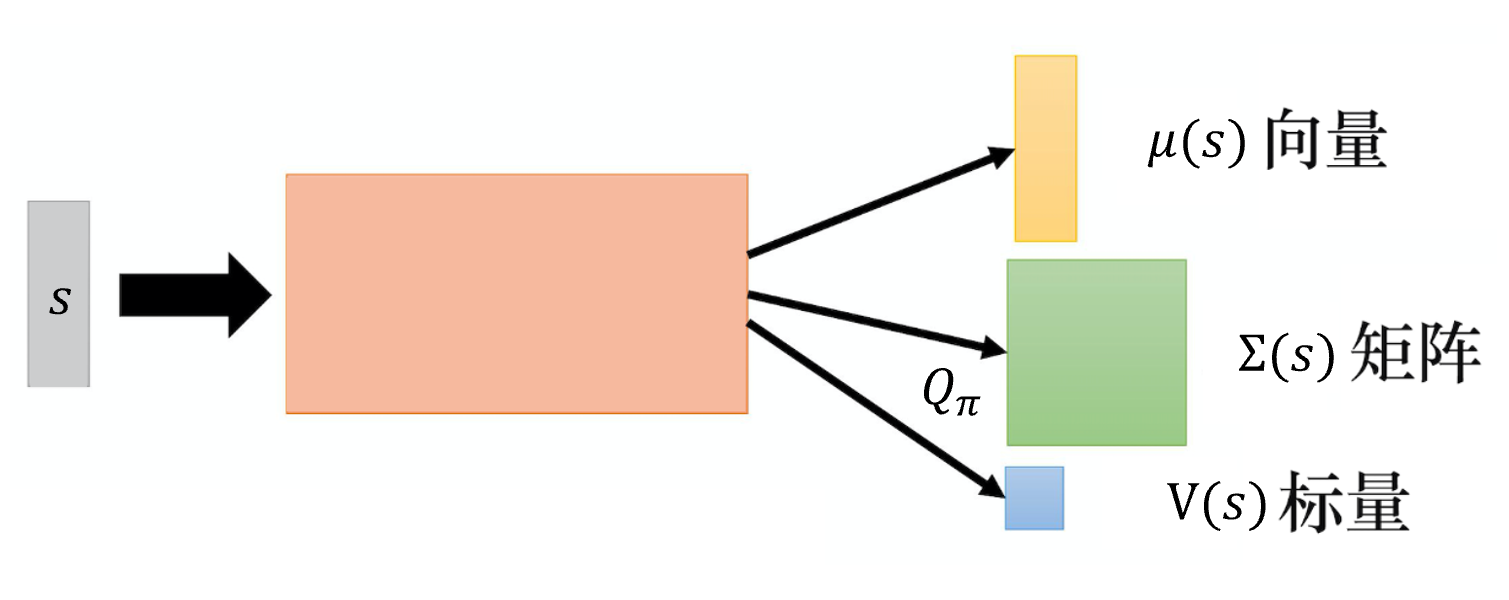
\includegraphics[width=0.5\linewidth]{res/ch8/8.2}
    \caption{方案 3:设计网络架构}
    \label{fig:fig8.2}
\end{figure} 

\subsection{方案 4:不使用深度Q网络}  

第4个方案就是不使用 深度Q网络,用 深度Q网络 处理连续动作是比较麻烦的。
如\figref{fig:fig8.3} 所示,我们将基于策略的方法------PPO 和基于价值的方法------深度Q网络 结合在一起,就可以得到演员-评论员的方法。

\begin{figure}[htpb]
  \centering
  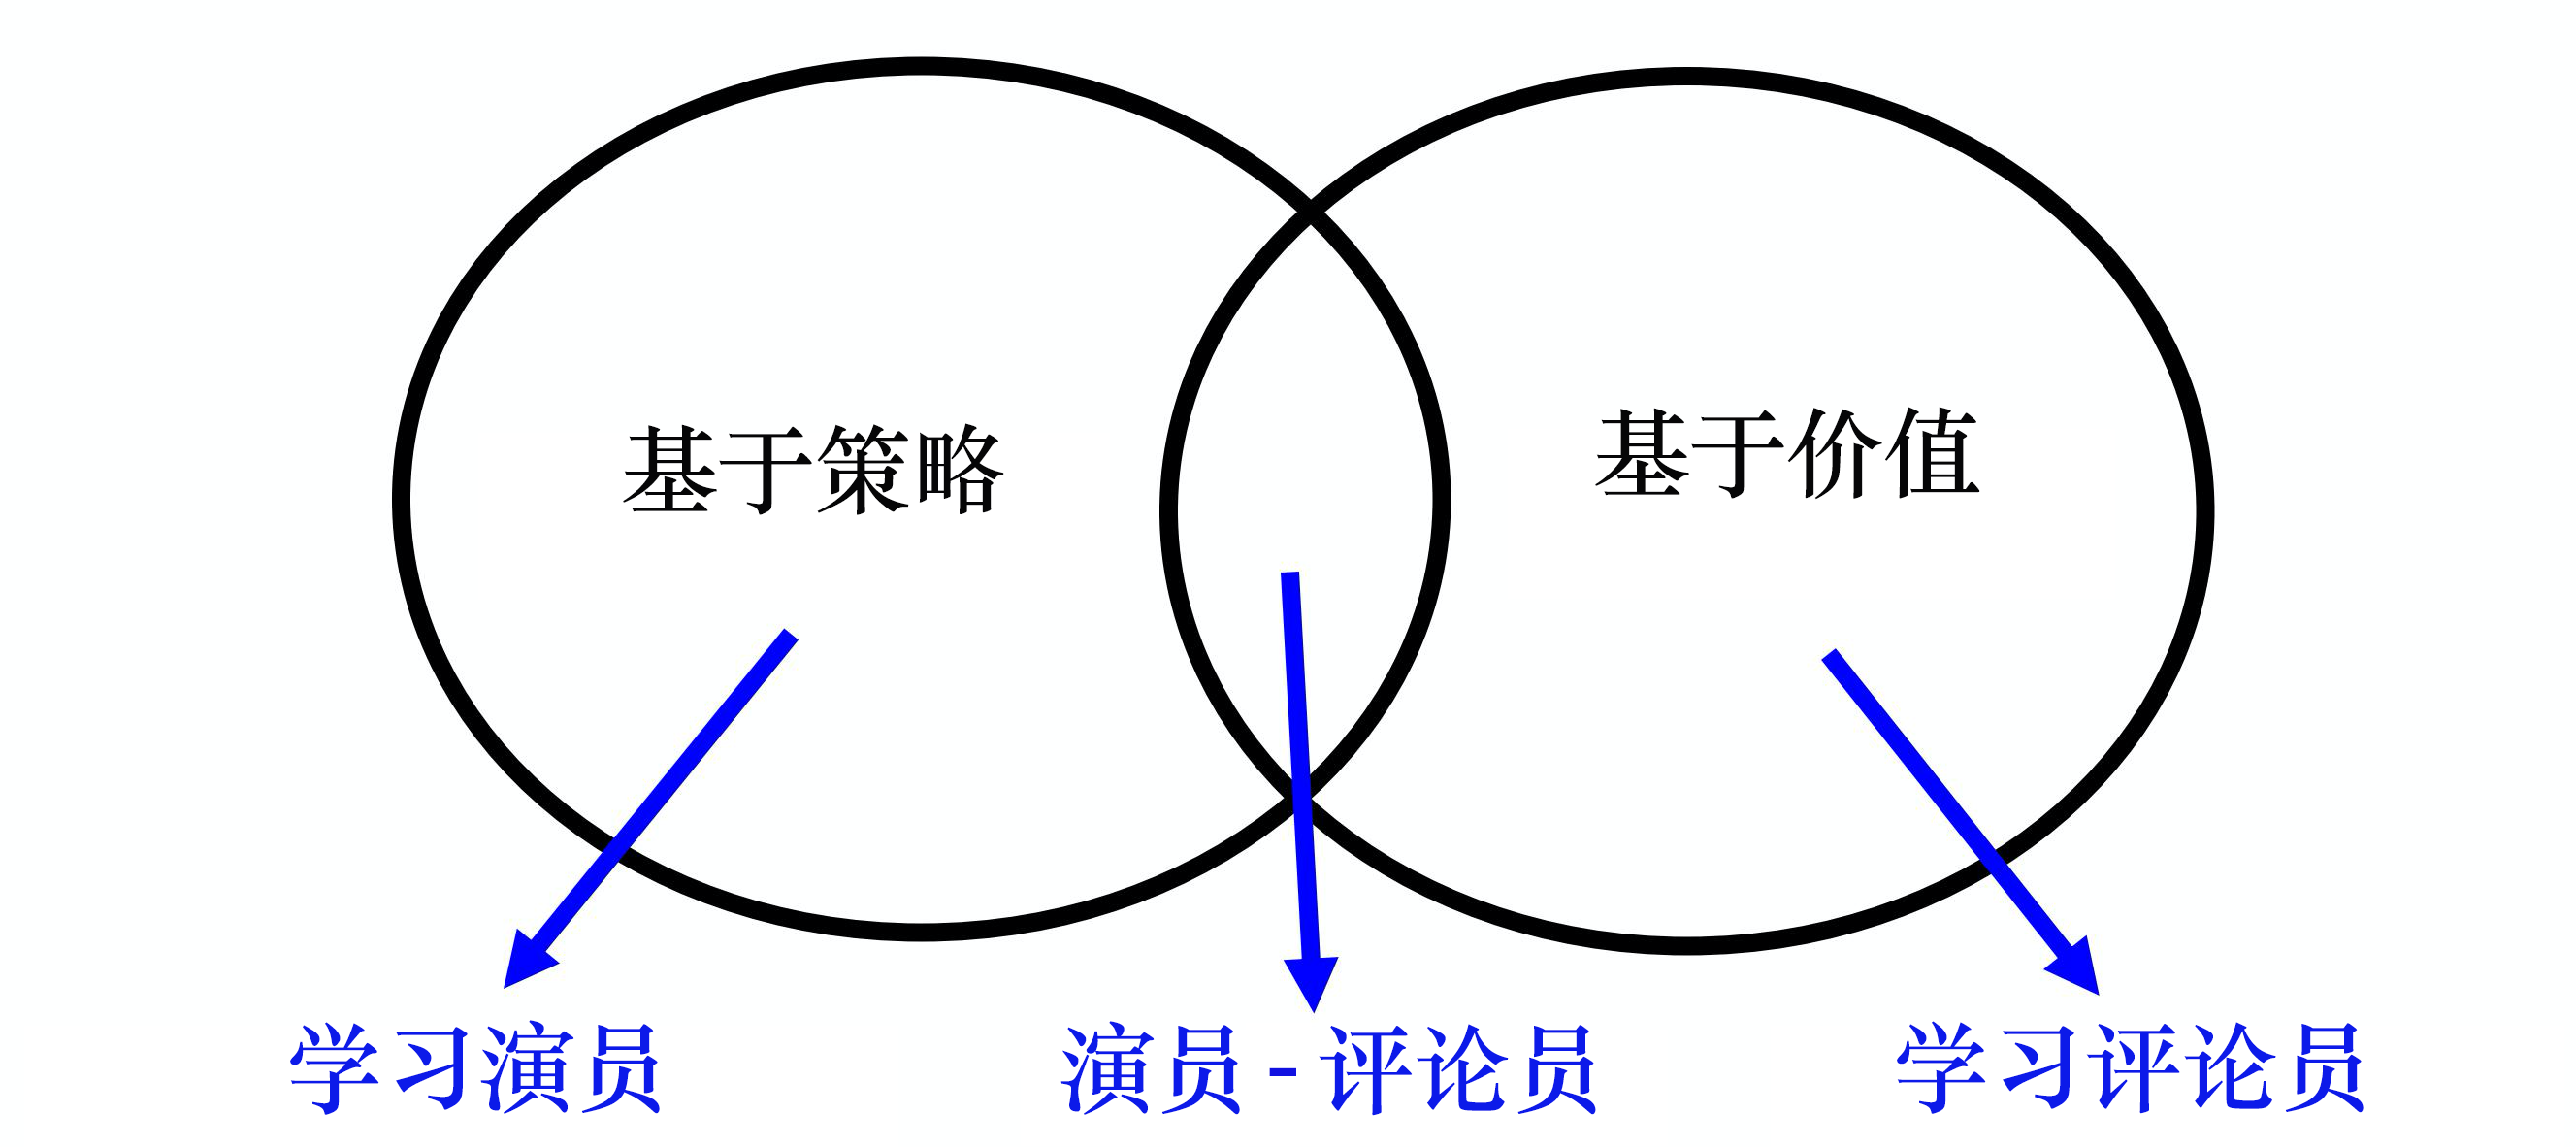
\includegraphics[width=0.5\linewidth]{res/ch8/8.3}
  \caption{方案 4:不使用 深度Q网络}
  \label{fig:fig8.3}
\end{figure}


\subsection{习题}

\kw{8-1} 深度Q网络相比基于策略梯度的方法为什么训练效果更好、更平稳?

\kw{8-2} 深度Q网络在处理连续动作时存在什么样的问题呢?对应的解决方法有哪些呢?
